% vim: foldmethod=marker foldlevel=0

% -----------------------------------------------------------------------------
% information
% -----------------------------------------------------------------------------

\def \docAuthor {\question{Name:}\answer{Answer Key}}
\def \docClass  {CPSC 120}
\def \docSchool {~}
\def \docTerm   {Spring 2014}
\def \docTitle  {worksheets}


% -----------------------------------------------------------------------------
% document setup
% -----------------------------------------------------------------------------
% {{{

\documentclass[12pt,letterpaper]{article}

\usepackage[includehead,
            includefoot,
            margin=1in,
            top=.25in,
            headheight=.75in,
            headsep=.25in,
            footskip=.25in,
           ]{geometry}

\usepackage[fleqn]{amsmath}
\usepackage{amssymb}
\usepackage{array}
\usepackage{enumitem}
\usepackage{fancybox}
\usepackage{fancyhdr}
\usepackage{l3regex}
\usepackage{mathtools}
\usepackage{minted}
\usepackage{multicol}
\usepackage{tikz}
\usepackage[normalem]{ulem}
\usepackage{url}
\usepackage{xcolor}


% text ------------------------------------------------------------------------

\binoppenalty = 10000  % never break next to a binary operator
\relpenalty   = 10000  % never break next to a relation operator

\setlength{\parindent}{0em}
\setlength{\parskip}{1ex}

\setlist[itemize]{nosep,itemsep=.5ex,parsep=.5ex}

% math ------------------------------------------------------------------------

\setlength{\mathindent}{1cm}

% - "\begin{document}" resets these values, so they have to be treated
%   specially
\AtBeginDocument{
  \setlength{\abovedisplayskip}{1.5ex plus .5ex minus .5ex}
  \setlength{\belowdisplayskip}{1.5ex plus .5ex minus .5ex}
}

% source code -----------------------------------------------------------------

\usemintedstyle{solarizedlight}

\fvset{samepage=true,frame=single,rulecolor=\color{.!30},framesep=2mm}

% header and footer -----------------------------------------------------------

\pagestyle{fancy}

\lhead{{\answer{\color{.}}\docClass}}
\rhead{{\answer{\color{.}}\docTitle}}
\cfoot{{\answer{\color{.}}\thepage}}
\renewcommand{\headrule}{{\answer{\color{red}}\hrule height 0.4pt}}
\renewcommand{\footrule}{{\answer{\color{red}}\hrule height 0.4pt}}

\fancypagestyle{firstpage}{
  \fancyhead[L]{{\answer{\color{red}}\docAuthor}
                {\answer{\color{.}}\\\docClass}}
  \fancyhead[C]{{\answer{\color{.}}\docSchool\\}}
  \fancyhead[R]{{\answer{\color{.}}\docTerm\\\docTitle}}
}


% -----------------------------------------------------------------------------
% macros
% -----------------------------------------------------------------------------

% abbreviations ---------------------------------------------------------------

\def \<{\langle}
\def \>{\rangle}

\def \ε{\varepisilon}
\def \θ{\vartheta}
\def \κ{\varkappa}
\def \π{\varpi}
\def \ρ{\varrho}
\def \σ{\varsigma}
\def \φ{\varphi}

\def \Γ{\varGamma}
\def \Δ{\varDelta}
\def \Θ{\varTheta}
\def \Λ{\varLambda}
\def \Ξ{\varXi}
\def \Π{\varPi}
\def \Σ{\varSigma}
\def \Υ{\varUpsilon}
\def \Φ{\varPhi}
\def \Ψ{\varPsi}
\def \Ω{\varOmega}

% special characters ----------------------------------------------------------

\catcode `α = \active \let α \alpha
\catcode `β = \active \let β \beta
\catcode `γ = \active \let γ \gamma
\catcode `δ = \active \let δ \delta
\catcode `ε = \active \let ε \epsilon
\catcode `ζ = \active \let ζ \zeta
\catcode `η = \active \let η \eta
\catcode `θ = \active \let θ \theta
\catcode `ι = \active \let ι \iota
\catcode `κ = \active \let κ \kappa
\catcode `λ = \active \let λ \lambda
\catcode `μ = \active \let μ \mu
\catcode `ν = \active \let ν \nu
\catcode `ξ = \active \let ξ \xi
\catcode `ο = \active \let ο o
\catcode `π = \active \let π \pi
\catcode `ρ = \active \let ρ \rho
\catcode `σ = \active \let σ \sigma
\catcode `τ = \active \let τ \tau
\catcode `υ = \active \let υ \upsilon
\catcode `φ = \active \let φ \phi
\catcode `χ = \active \let χ \chi
\catcode `ψ = \active \let ψ \psi
\catcode `ω = \active \let ω \omega

\catcode `Α = \active \let Α A
\catcode `Β = \active \let Β B
\catcode `Γ = \active \let Γ \Gamma
\catcode `Δ = \active \let Δ \Delta
\catcode `Ε = \active \let Ε E
\catcode `Ζ = \active \let Ζ Z
\catcode `Η = \active \let Η H
\catcode `Θ = \active \let Θ \Theta
\catcode `Ι = \active \let Ι I
\catcode `Κ = \active \let Κ K
\catcode `Λ = \active \let Λ \Lambda
\catcode `Μ = \active \let Μ M
\catcode `Ν = \active \let Ν N
\catcode `Ξ = \active \let Ξ \Xi
\catcode `Ο = \active \let Ο O
\catcode `Π = \active \let Π \Pi
\catcode `Ρ = \active \let Ρ P
\catcode `Σ = \active \let Σ \Sigma
\catcode `Τ = \active \let Τ T
\catcode `Υ = \active \let Υ \Upsilon
\catcode `Φ = \active \let Φ \Phi
\catcode `Χ = \active \let Χ X
\catcode `Ψ = \active \let Ψ \Psi
\catcode `Ω = \active \let Ω \Omega

% }}}
% other -----------------------------------------------------------------------

% - sometimes a "\par", especially at the end of a block, is necessary to
%   prevent an extra (empty) paragraph from appearing in the output
% - `\color{.!50}` means 50 percent of the current color

     \def \note     #1{{\color{.!50}#1\par}}
\long\def \longnote #1{{\color{.!50}#1\par}}

\def \mysection #1{%
  \newpage \thispagestyle{firstpage}
  \section{#1}
}

\def \ssFix    {\filbreak\subsection*{Fix the Broken Code}}
\def \ssTrace  {\filbreak\subsection*{Trace the Working Code}}
\def \ssScope  {\filbreak\subsection*{Circle the Variables' Scopes}}
\def \ssMemory {\filbreak\subsection*{Fill in the Memory}}

\def \codeFix #1{%
  \filbreak
  \question{
    \inputminted{c++}{./code/#1.cpp} \vspace{-6ex}
  } \answer{
    \inputminted{c++}{./code/#1.answer.cpp} \vspace{-6ex}
    \inputminted{diff}{./code/#1.answer.cpp.diff} \vspace{-6ex}
    \inputminted{text}{./code/#1.answer.cpp.output} \vspace{-6ex}
  }
}

\def \codeTrace #1{%
  \filbreak
  \inputminted{c++}{./code/#1.cpp} \vspace{-6ex}
  \question{
  } \answer{
    \inputminted{text}{./code/#1.cpp.output} \vspace{-6ex}
  }
}

\def \codeScope #1{%
  \filbreak
  \inputminted{c++}{./code/#1.cpp} \vspace{-6ex}
  \question{
  } \answer{
    \inputminted{text}{./code/#1.cpp.output} \vspace{-6ex}
  }
}

\def \codeMemory #1{%
  \filbreak
  \vspace{2ex}
  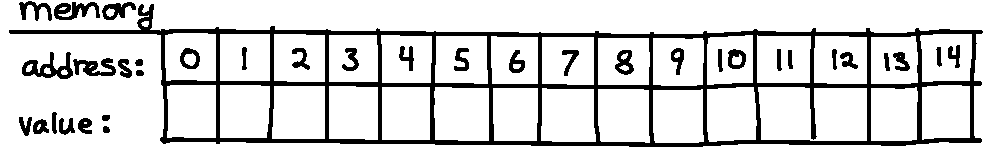
\includegraphics{./images/memory-0}
  \vspace{-2ex}
  \inputminted[frame=none,fontsize=\large]{c++}{./code/#1.cpp}
  \newpage
}


% -----------------------------------------------------------------------------
% document
% -----------------------------------------------------------------------------

\begin{document}


\newpage \thispagestyle{firstpage}
\section*{Instructions}
For a each topic (if applicable) there are 4 sections:

\ssFix
Modify the code in the cleanest (and preferably shortest) way possible, so that
it will compile and run without errors or warnings.

\ssTrace
Trace through the execution of the code, keeping track of the value of each
variable at each point in time, and the final output that the program produces.

\ssScope
Circle the scope of the given variable -- i.e., circle the part of the code in
which the variable ``exists''.  A good test, if you're not sure, is: if you
inserted a statement to \verb!cout! the variable at a given point in the code,
would any errors be produced?

\ssMemory
Fill in (or draw) a picture representing the computer memory, showing how the
variables might be allocated, and whether they have an assigned value, or are
uninitialized (use \verb!?! for ``uninitialized'').


\mysection{Variables and Assignment}

\ssFix
\codeFix{1-fix-1}
\codeFix{1-fix-2}
\newpage

\ssTrace
\codeTrace{1-trace-1}
\codeTrace{1-trace-2}
\newpage

\ssScope
\codeScope{1-scope-1}
\codeScope{1-scope-2}
\newpage

\ssMemory
\codeMemory{1-memory-1}


\mysection{Data Types and Expressions}
% TODO

\ssFix
\ssTrace
\ssScope
\ssMemory


\mysection{If and If-Else}
% TODO
% - *all* the different forms they can take

\ssFix
\ssTrace
\ssScope
\ssMemory


\mysection{Boolean Expressions}
% TODO:
% - evaluating by hand

\ssFix
\ssTrace
\ssScope
\ssMemory


\mysection{Predefined Functions}
% TODO
% - header files
% - usage
% - rand()
% - pow()

\ssFix
\ssTrace
\ssScope
\ssMemory


\mysection{Loops}
% TODO: for, while, do-while
% - tracing
% - correspondence between the different types

\ssFix
\ssTrace
\ssScope
\ssMemory


\mysection{Arrays}
% TODO
% - declaring
%   - uninitialized
%   - initialized
% - initializing with loops
% - initializing with cin
% - accessing a single element
% - swapping elements

\ssFix
\ssTrace
\ssScope
\ssMemory


\mysection{Selection Sort}
% TODO

\ssFix
\ssTrace
\ssScope
\ssMemory


\end{document}

